\documentclass[aspectratio=169,10pt]{beamer}
\usepackage[T1]{fontenc}
\usepackage[utf8]{inputenc}
\usepackage{lmodern}
\usepackage{amsmath,amssymb}
\usepackage{graphicx}
\usepackage{booktabs}
\usepackage{listings}
\usepackage{xcolor}
\usepackage{tikz}
\usetikzlibrary{arrows.meta,positioning,shapes.geometric,calc}
\usetheme{metropolis}
\metroset{progressbar=frametitle,sectionpage=none,numbering=fraction}

\title{Optimization Methods for Thermal Sciences}
\subtitle{A panorama of principles, algorithms and code}
\author{Whady Felipe Florez}
\institute{[Seminar / institution]}
\date{}

\lstdefinestyle{py}{
  language=Python,
  basicstyle=\ttfamily\fontsize{6.6}{7.7}\selectfont,
  keywordstyle=\color{blue!70!black}\bfseries,
  commentstyle=\color{gray},
  stringstyle=\color{orange!70!black},
  showstringspaces=false, breaklines=false, frame=single, framerule=0.3pt,
  tabsize=2, xleftmargin=0pt, xrightmargin=0pt, aboveskip=2pt, belowskip=2pt,
  morekeywords={as}
}
\lstset{style=py}
\newcommand{\codesz}[3]{\lstinputlisting[style=py,basicstyle=\ttfamily\fontsize{#1}{#2}\selectfont]{snippets/#3.py}}
\newcommand{\code}[1]{\codesz{6.6}{7.7}{#1}}
\newcommand{\grad}{\nabla}
\newcommand{\R}{\mathbb{R}}
\newcommand{\norm}[1]{\left\lVert #1\right\rVert}
\newcommand{\xs}{x^{\ast}}
\newcommand{\fig}[2][\linewidth]{\includegraphics[width=#1]{figs/#2}}
\setbeamertemplate{caption}{\insertcaption}

\begin{document}
\maketitle

\begin{frame}{Outline}
  \tableofcontents
\end{frame}

% =============================================================== 1
\section{Setting the stage}

\begin{frame}{Why optimization in the thermal sciences?}
  Every thermal design is a \textbf{compromise}: more insulation, more heat-exchanger area or more collector area costs money; too little wastes energy.
  \vspace{0.2cm}
  \begin{columns}[T]
    \begin{column}{0.52\textwidth}
      \begin{itemize}
        \item How thick should the insulation on a steam line be?
        \item How large a heat-recovery exchanger, and at what water flow?
        \item At what temperature should a solar field operate?
        \item Where should a temperature-sensitive part go on a hot board?
        \item Which $h$, $k$, $\varepsilon$ best fit my measured cooling curve?
      \end{itemize}
    \end{column}
    \begin{column}{0.44\textwidth}
      \begin{alertblock}{Today's goal}
        A \textbf{map} of the main families of methods, one clear \emph{picture} and one short \emph{code} per method, all on thermal problems.
      \end{alertblock}
      \small No heavy theory: what each method \textbf{does}, \textbf{when} it works and \textbf{when} it fails.
    \end{column}
  \end{columns}
\end{frame}

\begin{frame}{Anatomy of an optimization problem}
  \[ \min_{x\in\R^n}\ f(x)\qquad\text{subject to}\qquad g_j(x)\le 0,\quad h_i(x)=0 \]
  \begin{itemize}
    \item $x$: the \textbf{decision variables}, a \emph{vector} (thickness, area and flow, a position, \dots)
    \item $f(x)$: the \textbf{objective}: a single number to minimise (annual cost, temperature, exergy loss)
    \item $g(x)\le0,\ h(x)=0$: the \textbf{constraints} (maximum temperature, demand to be met, energy balance)
  \end{itemize}
  \begin{center}\small
  \begin{tabular}{llll}
    \toprule
    Problem & $x$ & $f(x)$ & constraint\\
    \midrule
    P1 insulation & $[t]$ & energy lost + insulation cost & --\\
    P2 component placement & $[x_1,x_2]$ & board temperature & inside the board\\
    P3 heat recovery & $[a,\,m]$ & area + pumping $-$ heat value & --\\
    P4 solar field & $[A,\ \Delta T]$ & area cost $-$ premium for hot heat & demand $\le A\,G\,\eta(\Delta T)$\\
    \bottomrule
  \end{tabular}
  \end{center}
\end{frame}

\begin{frame}{Four thermal test problems used throughout}
  \begin{columns}[T]
    \begin{column}{0.60\textwidth}
      \fig{fig_problems_overview.png}
    \end{column}
    \begin{column}{0.38\textwidth}
      \small
      \textbf{P1} \emph{1-D, unimodal}: golden section.\\[3pt]
      \textbf{P2} \emph{2-D, several valleys}: Metropolis, simulated annealing, Great Deluge.\\[3pt]
      \textbf{P3} \emph{2-D, smooth narrow valley}: gradient descent, Newton, dogleg, simplex.\\[3pt]
      \textbf{P4} \emph{2-D, constrained}: cutting plane, penalty and barrier.\\[6pt]
      \footnotesize Physical models are deliberately simple (closed-form), so the \emph{method} is the star, not the model.
    \end{column}
  \end{columns}
\end{frame}

\begin{frame}{P1: how thick should the insulation be?}
  \begin{columns}[T]
    \begin{column}{0.5\textwidth}
      \small
      Bare steam pipe ($r_1=5$ cm, 180\,$^\circ$C) in 20\,$^\circ$C air. Insulation of thickness $t$ ($k=0.045$ W/m\,K):
      \[ q'(t)=\frac{T_f-T_\infty}{\dfrac{\ln(r_2/r_1)}{2\pi k}+\dfrac{1}{2\pi r_2 h}},\quad r_2=r_1+t \]
      \[ f(t)=\underbrace{c_E\,q'(t)\,H}_{\text{energy lost}}+\underbrace{\mathrm{CRF}\,c_V\,\pi(r_2^2-r_1^2)}_{\text{insulation}} \]
      \footnotesize $H=8000$ h/yr, $c_E=0.04$ \$/kWh, $c_V=2500$ \$/m$^3$, CRF $=0.2$.
      \normalsize
      \begin{itemize}
        \item More insulation: less energy lost, more capital.
        \item Bare pipe: 161 \$/m/yr. Optimum: 31 \$/m/yr.
      \end{itemize}
    \end{column}
    \begin{column}{0.48\textwidth}
      \fig{fig_P1_cost.png}
    \end{column}
  \end{columns}
\end{frame}

\begin{frame}{P2: where to mount a temperature-sensitive component?}
  \begin{columns}[T]
    \begin{column}{0.46\textwidth}
      \small
      Thin board ($k=20$ W/m\,K, 2 mm) with 5 hot chips and 4 cooled clamps. Fin-type conduction gives, for each source $q_j$ (W):
      \[ T(x)=T_0+\sum_j\frac{q_j}{2\pi k\,t_b}\,K_0\!\bigl(m\,\|x-x_j\|\bigr) \]
      with $m=\sqrt{2h/(k\,t_b)}$ and $q_j<0$ for clamps.
      \begin{itemize}
        \item Goal: \textbf{minimise} $T(x)$, $x=[x_1,x_2]$ in the board.
        \item \textbf{Four local minima} (circled), one global: $(12.0,\,2.7)$\,cm, $24.4\,^\circ$C.
        \item The other three: 43--46\,$^\circ$C.
      \end{itemize}
    \end{column}
    \begin{column}{0.52\textwidth}
      \fig{fig_P2_landscape.png}
    \end{column}
  \end{columns}
\end{frame}

\begin{frame}{P3: heat-recovery exchanger (area and water flow)}
  \begin{columns}[T]
    \begin{column}{0.5\textwidth}
      \small
      Hot exhaust (20 kW/K, 250\,$^\circ$C) heats water of flow $m$ in a counter-flow exchanger of area $A=50\,a$ m$^2$ ($\varepsilon$--NTU):
      \[ \mathrm{NTU}=\frac{UA}{m c_p},\quad U=U_0\,m^{0.8},\quad Q=\varepsilon\,m c_p\,(T_h-T_c) \]
      \[ f(a,m)=\underbrace{c_A A}_{\text{area}}+\underbrace{c_p\,m^{2.8}}_{\text{pumping}}-\underbrace{c_Q\,Q}_{\text{value of heat}} \]
      \begin{itemize}
        \item Optimum: $A=220$ m$^2$, $m=1.44$ kg/s, $Q=1.35$ MW, net gain $93.6$ k\$/yr.
        \item A narrow curved valley: area and flow compensate each other.
        \item Hessian condition number $\approx 65$ at the optimum.
      \end{itemize}
    \end{column}
    \begin{column}{0.48\textwidth}
      \fig{fig_P3_landscape.png}
    \end{column}
  \end{columns}
\end{frame}

\begin{frame}{P4: solar collector field, constrained}
  \begin{columns}[T]
    \begin{column}{0.5\textwidth}
      \small
      Process heat of $Q_{dem}=100$ kW from collectors ($G=800$ W/m$^2$) with efficiency $\eta(\Delta T)=\eta_0-a_1\tfrac{\Delta T}{G}-a_2\tfrac{\Delta T^2}{G}$.
      \[ \min\ 5\,x_1-2\,x_2\quad\text{s.t.}\quad \underbrace{\frac{Q_{dem}}{G\,\eta(10x_2)}\cdot\frac1{100}-x_1}_{g(x)}\le0 \]
      $x_1=A/100$ m$^2$ (area cost 5 k\$/yr per unit), $x_2=\Delta T/10$ K (credit of 2 k\$/yr per unit: hotter heat is worth more).
      \begin{itemize}
        \item Optimum on the boundary: $A=275$ m$^2$, $\Delta T=59.4$ K, $\eta=0.454$.
        \item $g$ is \textbf{convex}: the feasible set is convex.
      \end{itemize}
    \end{column}
    \begin{column}{0.48\textwidth}
      \fig{fig_P4_feasible.png}
    \end{column}
  \end{columns}
\end{frame}

\begin{frame}[fragile]{The convention for all the code: $f(x)$ with $x$ a vector}
  \small Every method below receives \textbf{only a function of one vector}, a black box:
\begin{lstlisting}
def cost_insulation(x):                       # P1: x = [t]
    r2 = R1 + x[0]
    R_th = np.log(r2 / R1) / (2*np.pi*K_INS) + 1.0 / (2*np.pi*r2*H_OUT)
    energy  = (T_FLUID - T_AMB) / R_th / 1000.0 * HOURS * C_ENERGY
    capital = C_VOL * np.pi * (r2**2 - R1**2) * CRF
    return energy + capital

def temperature_board(x):                     # P2: x = [x1, x2]  (cm)
    d = np.sqrt(np.sum((x - SRC[:, :2])**2, axis=1) + R0**2)       # distance to every source
    return T_BASE + np.sum(SRC[:, 2] / (2*np.pi*K_PLATE*THK) * k0(M_FIN * d))

def cost_exchanger(x):                        # P3: x = [a, m]
    A, m = 50.0 * x[0], x[1]
    return (C_AREA*A + C_PUMP*m**2.8 - C_HEAT*exchanger_duty(x)/1000.0) / 1000.0
\end{lstlisting}
  Same signature for 1, 2 or 200 variables: \texttt{f(x)}. Methods never see the physics; they only call $f$.
\end{frame}

\begin{frame}{A map of the methods}
  \centering
  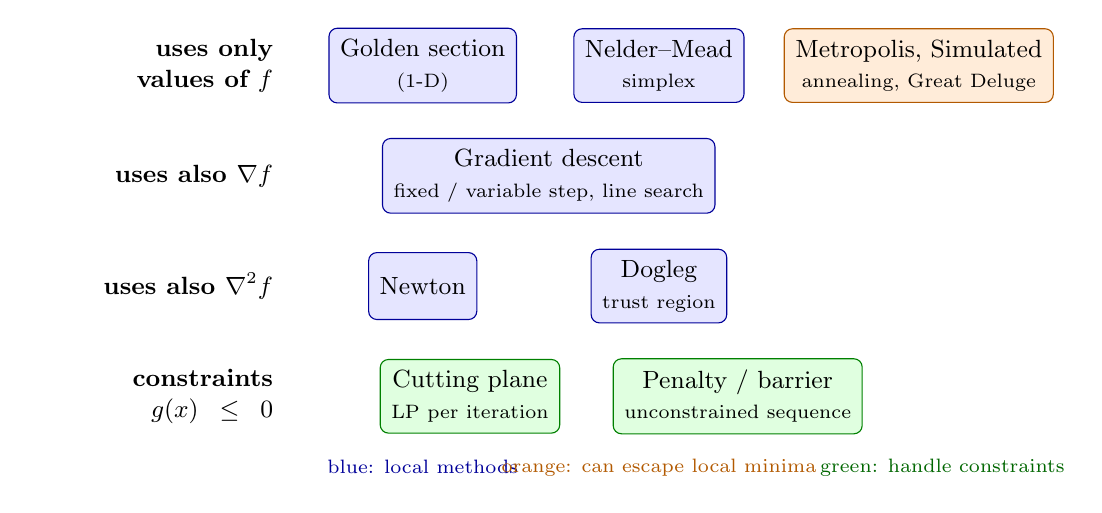
\begin{tikzpicture}[
      lab/.style={font=\small\bfseries, text width=3.0cm, align=right},
      box/.style={draw, rounded corners=3pt, align=center, minimum height=0.85cm, font=\small, inner sep=4pt},
      glob/.style={box, fill=orange!15, draw=orange!70!black},
      loc/.style={box, fill=blue!10, draw=blue!60!black},
      con/.style={box, fill=green!12, draw=green!50!black}]
    \node[lab] at (0,3.6) {uses only values of $f$};
    \node[loc] at (3.4,3.6) {Golden section\\ \scriptsize(1-D)};
    \node[loc] at (6.4,3.6) {Nelder--Mead\\ \scriptsize simplex};
    \node[glob] at (9.7,3.6) {Metropolis, Simulated\\ \scriptsize annealing, Great Deluge};
    \node[lab] at (0,2.2) {uses also $\grad f$};
    \node[loc] at (5.0,2.2) {Gradient descent\\ \scriptsize fixed / variable step, line search};
    \node[lab] at (0,0.8) {uses also $\grad^2 f$};
    \node[loc] at (3.4,0.8) {Newton};
    \node[loc] at (6.4,0.8) {Dogleg\\ \scriptsize trust region};
    \node[lab] at (0,-0.6) {constraints $g(x)\le 0$};
    \node[con] at (4.0,-0.6) {Cutting plane\\ \scriptsize LP per iteration};
    \node[con] at (7.4,-0.6) {Penalty / barrier\\ \scriptsize unconstrained sequence};
    \node[font=\scriptsize, text=blue!60!black] at (3.4,-1.5) {blue: local methods};
    \node[font=\scriptsize, text=orange!70!black] at (6.4,-1.5) {orange: can escape local minima};
    \node[font=\scriptsize, text=green!40!black] at (10.0,-1.5) {green: handle constraints};
  \end{tikzpicture}
\end{frame}

\begin{frame}{Local versus global: why the landscape matters}
  \begin{columns}[T]
    \begin{column}{0.5\textwidth}
      \begin{itemize}
        \item A \textbf{local} method stops in the valley where it starts. Start near $(23,8)$\,cm: it ends at \textbf{43\,$^\circ$C}, although $24$\,$^\circ$C exists elsewhere.
        \item Smooth \emph{unimodal} problems (P1, P3): local methods are enough, and the fastest ones win.
        \item \emph{Multimodal} problems (P2): we need a method that sometimes accepts a \textbf{worse} point.
      \end{itemize}
      \begin{alertblock}{Rule of thumb}
        First plot (or sample) $f$. If you see several valleys, think \textbf{global}; if one smooth valley, think \textbf{Newton-like}.
      \end{alertblock}
    \end{column}
    \begin{column}{0.48\textwidth}
      \fig{fig_P2_landscape.png}
    \end{column}
  \end{columns}
\end{frame}

% =============================================================== 2
\section{Golden-section search}

\begin{frame}{Golden section: the simplest method (1-D, no derivatives)}
  \begin{itemize}
    \item Assume $f$ is \textbf{unimodal} on $[a,b]$ (one valley). Evaluate two interior probes $x_1<x_2$.
    \item If $f(x_1)<f(x_2)$ the minimum is in $[a,x_2]$; otherwise in $[x_1,b]$. \textbf{Discard the rest.}
    \item Choose the probes at $x_1=b-r(b-a)$, $x_2=a+r(b-a)$ with $r=\frac{\sqrt5-1}{2}=0.618\dots$
  \end{itemize}
  \begin{alertblock}{Why the golden ratio?}
    With this $r$ one surviving probe lands \textbf{exactly} on a probe of the next iteration: only \textbf{one new evaluation} per iteration, and the bracket shrinks by $0.618$ each time.
  \end{alertblock}
  \small Thermal use: any one-parameter design with a single optimum (insulation thickness, fin length, optimal flow rate).
\end{frame}

\begin{frame}{Golden section on P1: iteration by iteration}
  \centering
  \includegraphics[height=6.5cm]{figs/fig_golden_iter.png}
\end{frame}

\begin{frame}{Golden section: the code}
  \code{golden}
  \small \texttt{f} takes a vector (\texttt{f(np.array([t]))}); \texttt{f1}, \texttt{f2} are \textbf{reused}, never recomputed.
\end{frame}

\begin{frame}{Golden section: result and cost}
  \begin{columns}[T]
    \begin{column}{0.48\textwidth}
      \small
      \begin{center}
      \begin{tabular}{lrr}
        \toprule
        & manual & \texttt{scipy} golden\\
        \midrule
        $t^\ast$ [cm] & 4.549 & 4.548\\
        $f(t^\ast)$ [\$/m/yr] & 31.2518 & 31.2518\\
        iterations & 16 & 20\\
        $f$ evaluations & 18 & 25\\
        \bottomrule
      \end{tabular}
      \end{center}
      Bracket $[0,15]$ cm $\to$ $0.1$ mm.
      \begin{itemize}
        \item Robust, no derivatives; linear convergence ($0.618$ per evaluation).
        \item Fails silently if $f$ has several valleys in the bracket.
      \end{itemize}
      \footnotesize \texttt{minimize\_scalar(method="golden")}
    \end{column}
    \begin{column}{0.5\textwidth}
      \fig{fig_golden_conv.png}
    \end{column}
  \end{columns}
\end{frame}

% =============================================================== 3
\section{Escaping local minima: Metropolis, annealing, Deluge}

\begin{frame}{The problem: a valley is not the best valley}
  \begin{columns}[T]
    \begin{column}{0.5\textwidth}
      \begin{itemize}
        \item P2: start at $x_0=(23,\,8)$ cm, in a shallow cold pocket near a clamp ($43.4\,^\circ$C).
        \item Any method that only accepts \textbf{improvements} (``greedy'') stays there: every neighbour is hotter.
        \item To reach the cold region near $(12,\,2.7)$ we must first \textbf{climb} through $\approx$55\,$^\circ$C.
      \end{itemize}
      \begin{alertblock}{Key idea}
        Accept an \textbf{uphill} move sometimes, with a probability that depends on how bad it is.
      \end{alertblock}
    \end{column}
    \begin{column}{0.5\textwidth}
      \fig{fig_P2_landscape.png}
    \end{column}
  \end{columns}
\end{frame}

\begin{frame}{The thermodynamic idea (Metropolis, 1953)}
  \begin{columns}[T]
    \begin{column}{0.55\textwidth}
      \begin{itemize}
        \item A system at temperature $T$ visits a state of energy $E$ with probability
        \[ p(E)\propto e^{-E/(k_BT)} \qquad\text{(Boltzmann)} \]
        \item \textbf{Metropolis} built a simple random walk whose visits follow exactly this law:
        \begin{itemize}
          \item propose a random move $x\to x'$, $\Delta E=f(x')-f(x)$;
          \item \textbf{accept} it if $\Delta E\le0$;
          \item otherwise accept with probability $e^{-\Delta E/T}$.
        \end{itemize}
        \item Here $f$ plays the role of energy and $T$ is a ``temperature'' in the units of $f$ ($^\circ$C for P2).
      \end{itemize}
    \end{column}
    \begin{column}{0.43\textwidth}
      \fig{fig_metropolis_prob.png}
    \end{column}
  \end{columns}
\end{frame}

\begin{frame}{Metropolis: the code}
  \code{metropolis}
\end{frame}

\begin{frame}{A chain at fixed $T$ samples the Boltzmann distribution}
  \centering
  \fig[0.80\linewidth]{fig_boltzmann_P1.png}\\[2pt]
  \small Check on P1: histogram of 150\,000 Metropolis steps (blue) against the theoretical $e^{-f/T}$ (orange).\\
  Low $T$: the chain hugs the minimum. High $T$: it wanders widely. \textbf{$T$ is the exploration knob.}
\end{frame}

\begin{frame}{Fixed temperature on P2: exploration versus exploitation}
  \centering
  \fig[0.97\linewidth]{fig_metropolis_P2.png}
  \begin{itemize}
    \item $T\approx0$ (greedy): stuck at 43.4\,$^\circ$C. $\;T=3$: crosses to the cold region and stays. $\;T=20$: accepts almost everything and never settles.
    \item Too cold = trapped; too hot = random walk. The right $T$ depends on the \textbf{barrier heights} of the problem.
  \end{itemize}
\end{frame}

\begin{frame}{Simulated annealing: cool the temperature as you go}
  \small
  A Metropolis chain with a \textbf{decreasing} temperature, as when a metal is cooled slowly into a low-energy lattice:
  $T_k=T_0\,\alpha^{k}$, $0<\alpha<1$. Hot $\to$ explores; cold $\to$ refines. Keep the \textbf{best point ever seen}.\\[8pt]
  \codesz{7.3}{8.6}{sa}
  \footnotesize Parameters: $T_0\approx$ barrier height, $\alpha$ such that $T_{end}$ is small, step $\approx$ feature size.
\end{frame}

\begin{frame}{Simulated annealing on P2}
  \begin{columns}[T]
    \begin{column}{0.5\textwidth}\fig{fig_sa_path.png}\end{column}
    \begin{column}{0.48\textwidth}\fig{fig_sa_schedule.png}\end{column}
  \end{columns}
  \small $T_0=20\,^\circ$C, $\alpha=0.997$, 2000 steps, step size 1 cm. Start $(23,8)$ $\to$ best $24.4\,^\circ$C at $(12.0,\,2.7)$.
\end{frame}

\begin{frame}{Great Deluge (Dueck, 1993): a flood instead of a temperature}
  \begin{columns}[T]
    \begin{column}{0.33\textwidth}
      \footnotesize
      \begin{itemize}
        \item Picture a hiker in a landscape while a flood level \textbf{sinks} steadily.
        \item Accept \textbf{any} move whose $f$ is below the level: no probabilities, no $T$.
        \item The level falls by a fixed ``rain'' each step, from a high start to a \textbf{target} value.
        \item The region shrinks into separate ponds; the walker ends in the one it is in.
      \end{itemize}
      \begin{alertblock}{Parameters}
        start level, \textbf{target}, step: the target is an \emph{engineering goal} (here 26\,$^\circ$C).
      \end{alertblock}
    \end{column}
    \begin{column}{0.65\textwidth}
      \fig{fig_deluge.png}
    \end{column}
  \end{columns}
\end{frame}

\begin{frame}{Great Deluge: the code}
  \codesz{7.3}{8.8}{deluge}\vspace{4pt}
  \small Note how short it is: one comparison \texttt{f\_new <= level} replaces the whole Metropolis probability.
\end{frame}

\begin{frame}{Head to head on P2 (same start, same budget)}
  \begin{columns}[T]
    \begin{column}{0.62\textwidth}
      \fig{fig_stochastic_compare.png}
    \end{column}
    \begin{column}{0.36\textwidth}
      \small
      \begin{itemize}
        \item 60 seeds, 2000 evaluations each, start $(23,8)$, step 1 cm; success: $f<26\,^\circ$C.
        \item Greedy: \textbf{never} escapes.
        \item If we \textbf{remember the best point}, any $T$ high enough to cross the barriers finds the cold region (95--100\%).
        \item But \textbf{where the walker ends} is another story: only SA \emph{ends} cold (75\%).
        \item Great Deluge: 63\% / 42\%.
      \end{itemize}
      \footnotesize Judge stochastic methods over many seeds, never one run.
    \end{column}
  \end{columns}
\end{frame}

\begin{frame}{What does the temperature knob really do?}
  \centering
  \fig[0.80\linewidth]{fig_T_sweep.png}
  \small
  \begin{itemize}
    \item \textbf{Best visited:} fixed $T\ge3$ already finds the cold region; SA needs a hot enough start ($T_0\gtrsim10$), because it cools while exploring. Too cold ($T\le1$): trapped.
    \item \textbf{Final position:} a fixed-$T$ chain ends wherever thermal noise puts it (best $\approx40\%$ at $T=2$--3, nearly 0 when hotter). SA's final state is good ($\approx80\%$) \emph{without} bookkeeping, because it cools into the minimum.
  \end{itemize}
\end{frame}

\begin{frame}[fragile]{In \texttt{scipy} and in practice}
\begin{lstlisting}
from scipy.optimize import dual_annealing
res = dual_annealing(temperature_board, bounds=[(0, 24), (0, 16)], seed=0, maxfun=2000)
print(res.x, res.fun)          # -> [12.04  2.70]   24.38 C
\end{lstlisting}
  \begin{itemize}
    \item \texttt{dual\_annealing} (generalised SA plus a local polish) reaches the same optimum as our manual code.
    \item Practical advice: choose \textbf{step} from the feature size of $f$, $T_0$ from a typical \textbf{barrier}, $T_{end}$ from the resolution you need; run \textbf{many seeds}; keep the best point; finish with a local method.
    \item Cost: thousands of evaluations; use them when $f$ is cheap, derivatives unavailable, or valleys abound.
  \end{itemize}
\end{frame}
